%% ============================================================
%%  QSAR Project Presentation (Less Technical)
%%  Source: docs/REPO_STRUCTURE_AND_OUTPUTS.txt
%%          docs/TERMS_AND_WORKFLOW_EXPLAINED.txt
%% ============================================================
\documentclass[aspectratio=169,10pt]{beamer}

% Theme
\usetheme{Madrid}
\usecolortheme{whale}
\setbeamertemplate{navigation symbols}{}
\setbeamertemplate{footline}[page number]

% Packages
\usepackage{booktabs}
\usepackage{tabularx}
\usepackage{graphicx}
\usepackage{xcolor}
\usepackage{amsmath,amssymb}
\usepackage{tikz}
\usetikzlibrary{arrows.meta,positioning,shapes.geometric}
\usepackage{hyperref}
\hypersetup{colorlinks=false}

% Colors
\definecolor{mainblue}{RGB}{0,82,147}
\definecolor{accent}{RGB}{0,150,136}
\definecolor{warn}{RGB}{220,90,40}
\definecolor{softgray}{RGB}{245,245,245}

\setbeamercolor{palette primary}{bg=mainblue, fg=white}
\setbeamercolor{palette secondary}{bg=accent, fg=white}
\setbeamercolor{structure}{fg=mainblue}

% TikZ styles
\tikzstyle{pstep}=[rectangle,rounded corners=4pt,draw=mainblue,fill=mainblue!10,
                  minimum height=0.9cm,text width=2.9cm,align=center,font=\scriptsize]
\tikzstyle{arrow}=[-{Stealth[length=5pt]},thick,draw=mainblue]
\tikzstyle{gatebox}=[rectangle,rounded corners=4pt,draw=accent,fill=accent!12,
                  minimum height=0.9cm,text width=3.0cm,align=center,font=\scriptsize]

% Title
\title[QSAR Pipeline Overview]{QSAR + REINVENT Pipeline Overview\\
Simple, Process-Focused Project Presentation}
\subtitle{Based on the comprehensive report and repository structure documents}
\author{QSAR Project Team}
\institute{Computational Drug Discovery}
\date{\today}

\begin{document}

\begin{frame}[plain]
  \titlepage
\end{frame}

\begin{frame}{What this presentation covers}
  \tableofcontents
\end{frame}

% ============================================================
\section{QSAR to translation walkthrough}
% ============================================================

\begin{frame}{Pipeline order used in this project}
  \begin{center}
    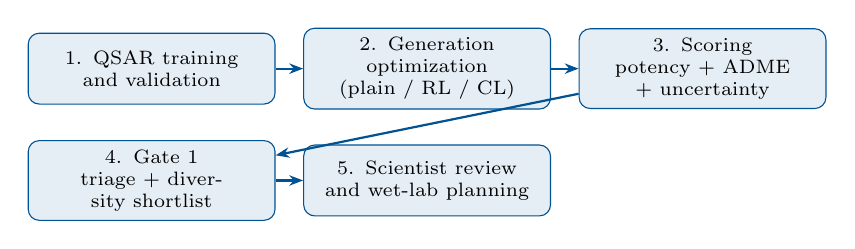
\begin{tikzpicture}[node distance=0.45cm and 0.35cm]
      \node[pstep] (q)  {1. QSAR training\\and validation};
      \node[pstep,right=of q] (g)  {2. Generation optimization\\(plain / RL / CL)};
      \node[pstep,right=of g] (s)  {3. Scoring\\potency + ADME + uncertainty};
      \node[pstep,below=of q] (g1) {4. Gate 1\\triage + diversity shortlist};
      \node[pstep,right=of g1] (w) {5. Scientist review\\and wet-lab planning};

      \draw[arrow] (q)--(g);
      \draw[arrow] (g)--(s);
      \draw[arrow] (s)--(g1);
      \draw[arrow] (g1)--(w);
    \end{tikzpicture}
  \end{center}

  \vspace{4pt}
  \begin{block}{Why this ordering}
    Learn from known data first (QSAR), optimize generation next, then use
    Gate 1 triage and diversity control before selecting compounds for lab planning.
  \end{block}
\end{frame}

\begin{frame}{Data acquisition \(\rightarrow\) deployment lifecycle}
  \small
  \begin{columns}[T]
    \column{0.48\textwidth}
      \begin{block}{1) Data acquisition}
        Experimental series data (C/E + historical labels), SMILES cleaning,
        canonicalization, and deduplication.
      \end{block}
      \begin{block}{2) Modeling}
        Descriptor generation + model selection for potency prediction.
        Best potency model: \textbf{RDKit + KNN}.
      \end{block}
      \begin{block}{3) Evaluation}
        Held-out validation on Series C and prospective ranking on Series E.
      \end{block}
    \column{0.48\textwidth}
      \begin{block}{4) Testing (in-silico pipeline testing)}
        REINVENT generation campaigns, automated scoring, and
        Gate 1 shortlist construction for downstream review.
      \end{block}
      \begin{block}{5) Deployment / operational use}
        Final ranked workbook is produced for chemistry/biology teams to
        choose wet-lab candidates and plan experiments.
      \end{block}
      \begin{exampleblock}{Key current results}
        Series C: MAE \textbf{0.118}, \(R^2=\textbf{0.887}\)\\
        Gate 1 shortlist: \textbf{200} candidates
      \end{exampleblock}
  \end{columns}
\end{frame}

\begin{frame}{Step 1: QSAR model training and key result}
  \begin{columns}[T]
    \column{0.54\textwidth}
      \begin{block}{How QSAR is built}
        \begin{enumerate}
          \item Clean and standardize molecular structures.
          \item Compute descriptor families (RDKit/ECFP/MACCS/Mordred).
          \item Train multiple regressors and compare on held-out data.
          \item Keep best model for primary IC\(_{50}\) prediction.
        \end{enumerate}
      \end{block}
    \column{0.44\textwidth}
      \begin{block}{Key performance (current artifact)}
        \small
        Best model:\\
        \textbf{RDKit + KNN}\\
        \(R^2 \approx 0.887\)

        \vspace{4pt}
        Additional positive-\(R^2\) models used for uncertainty:
        \begin{itemize}
          \item ECFP\_r3 + KNN
          \item RDKit + Decision Tree
          \item RDKit + LGBM
          \item RDKit + Extra Trees
        \end{itemize}
      \end{block}
  \end{columns}
\end{frame}

\begin{frame}{Where QSAR test outputs are saved (Series C/E)}
  \small
  \begin{block}{Primary C/E prediction files}
    {\scriptsize\texttt{outputs/qsar/core\_predictions/SeriesC\_test\_with\_predictions.csv}}\\
    {\scriptsize\texttt{outputs/qsar/core\_predictions/SeriesE\_with\_predictions.csv}}
  \end{block}

  \begin{block}{Manifest files}
    {\scriptsize\texttt{outputs/qsar/manifests/qsar\_outputs\_manifest.csv}}\\
    {\scriptsize\texttt{outputs/qsar/manifests/additional\_qsar\_outputs\_manifest.csv}}
  \end{block}

  \begin{exampleblock}{What each contains}
    \begin{itemize}
      \item Canonical structures and identifiers
      \item Predicted \(pIC_{50}\) and predicted IC\(_{50}\) (\(\mu\)M)
      \item Source/series metadata and downstream analysis fields
    \end{itemize}
  \end{exampleblock}
\end{frame}

\begin{frame}{Series C and E testing: key QSAR outputs}
  \begin{columns}[T]
    \column{0.48\textwidth}
      \begin{block}{Series C (test set)}
        \begin{itemize}
          \item Total rows: \textbf{6}
          \item Rows with measured pIC\(_{50}\): \textbf{5}
          \item MAE (pIC\(_{50}\)): \textbf{0.118}
          \item \(R^2\): \textbf{0.887}
        \end{itemize}
      \end{block}
    \column{0.48\textwidth}
      \begin{block}{Series E (prediction set)}
        \begin{itemize}
          \item Total rows predicted: \textbf{6}
          \item Predicted pIC\(_{50}\) range: \textbf{4.467 to 5.132}
          \item Predicted IC\(_{50}\) range: \textbf{7.38 to 34.11 \(\mu\)M}
        \end{itemize}
      \end{block}
  \end{columns}

  \vspace{4pt}
  \begin{alertblock}{Interpretation for presentation}
    Series C confirms model quality on known test compounds; Series E provides
    prospective potency ranking for compounds without direct fitted labels.
  \end{alertblock}
\end{frame}

\begin{frame}{Step 2: Generation optimization (plain, RL, CL)}
  \begin{columns}[T]
    \column{0.48\textwidth}
      \begin{block}{How optimization works}
        \begin{itemize}
          \item \textbf{Plain}: broad exploration from prior model.
          \item \textbf{RL}: sample \(\rightarrow\) score \(\rightarrow\) update agent.
          \item \textbf{CL}: staged objectives from easier to stricter targets.
        \end{itemize}
      \end{block}
      \begin{exampleblock}{Why CL is important}
        More stable learning, fewer invalid molecules,
        better quality at convergence.
      \end{exampleblock}
    \column{0.48\textwidth}
      \begin{block}{Used in this project}
        Families/modes were run across campaigns, then all sampled outputs
        were passed through one consistent scoring and gating workflow.

        \vspace{3pt}
        Typical path:\\
        {\scriptsize\texttt{reinvent\_integration/results/}}\\
        {\scriptsize\texttt{<family\_mode>/samples.csv}}
      \end{block}
  \end{columns}
\end{frame}

\begin{frame}{Step 3: Scoring and ranking logic}
  \small
  \begin{block}{Scoring stack}
    Validate SMILES \(\rightarrow\) descriptors \(\rightarrow\) potency prediction
    \(\rightarrow\) ADME/risk enrichment \(\rightarrow\) uncertainty estimation
    \(\rightarrow\) gate-ready output fields.
  \end{block}

  \begin{columns}[T]
    \column{0.50\textwidth}
      \begin{block}{Gate 1 triage equation}
      \[
\text{triage}=0.35P+0.15S+0.15L+0.10M+0.10H+0.15T
      \]
      \(P\): potency, \(S\): solubility, \(L\): cLogP window,\\
      \(M\)/\(H\): clearance terms, \(T\): half-life.
      \end{block}
    \column{0.46\textwidth}
      \begin{block}{Scored output location}
        \texttt{outputs/generated/<family>/<mode>/}\\
        CSV + Excel with structures and fields used by gates.
      \end{block}
  \end{columns}
\end{frame}

\begin{frame}{How uncertainty is controlled in ranking}
  \small
  \begin{block}{Uncertainty calculation}
    Up to 5 positive-\(R^2\) models predict each molecule.
    \[
      \mu = \frac{1}{k}\sum_{i=1}^{k}\hat{y}_i,
      \quad
      \sigma = \sqrt{\frac{1}{k-1}\sum_{i=1}^{k}(\hat{y}_i-\mu)^2}
    \]
    Lower \(\sigma\) means higher confidence.
  \end{block}

  \begin{columns}[T]
    \column{0.48\textwidth}
      \begin{block}{Control mechanism}
        \begin{itemize}
          \item Primary potency remains best model output.
          \item Uncertainty columns are retained for analysis and confidence review.
          \item Confidence columns are carried into final ranking.
        \end{itemize}
      \end{block}
    \column{0.48\textwidth}
      \begin{alertblock}{Practical effect}
        Reduces false positives that look strong in one model but unstable
        across the ensemble.
      \end{alertblock}
  \end{columns}
\end{frame}

\begin{frame}{Step 4: Active shortlist output (Gate 1)}
  \begin{columns}[T]
    \column{0.50\textwidth}
      \begin{block}{What Gate 1 optimizes}
        \begin{itemize}
          \item Potency + ADME multi-objective triage
          \item Scaffold-diverse shortlist selection
      \begin{alertblock}{Current run note}
        \texttt{pred\_pIC50\_uncertainty} = 0 in the current scored outputs,
        indicating a single effective model is being used for potency prediction.
        Ensemble uncertainty is available when multiple positive-\(R^2\) models
        are active during scoring.
      \end{alertblock}
          \item Consistent ranking fields for review
          \item Decision-ready workbook export
        \end{itemize}
      \end{block}
    \column{0.46\textwidth}
      \begin{block}{Current outputs}
        \texttt{outputs/hybrid\_stage/}\\
        \texttt{gate1/}\\
        \texttt{gate1\_shortlist.xlsx}
      \end{block}
      \begin{exampleblock}{Current count}
        Gate 1 shortlist: \textbf{200}
      \end{exampleblock}
  \end{columns}
\end{frame}

\begin{frame}{What was done and what you can present}
  \small
  \begin{enumerate}
    \item Built QSAR with best-performing potency model and ensemble uncertainty.
    \item Ran REINVENT generation campaigns across families and optimization modes.
    \item Scored all generated molecules with one consistent scoring pipeline.
    \item Applied Gate 1 triage ranking and scaffold-diverse shortlist selection.
    \item Produced ranked Excel outputs for medicinal-chemistry review and lab planning.
  \end{enumerate}

  \vspace{4pt}
  \begin{block}{Final narrative}
    \textbf{QSAR learns}, \textbf{REINVENT explores/optimizes},
    and \textbf{Gate 1 delivers an actionable shortlist}.
  \end{block}
\end{frame}

% ============================================================
\section{QSAR Modeling (Detailed)}
% ============================================================

\begin{frame}{QSAR modeling flowchart: data acquisition to model artifact}
  \begin{center}
    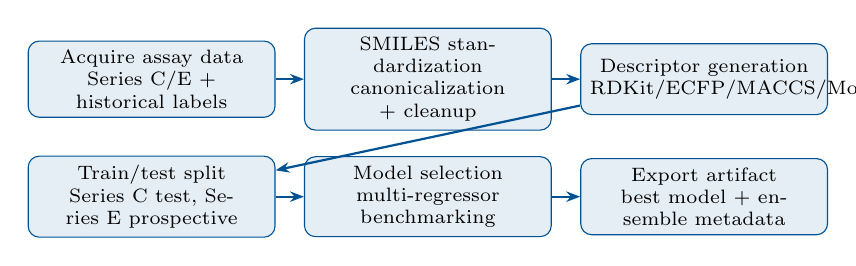
\begin{tikzpicture}[node distance=0.48cm and 0.36cm]
      \node[pstep] (d1) {Acquire assay data\\Series C/E + historical labels};
      \node[pstep,right=of d1] (d2) {SMILES standardization\\canonicalization + cleanup};
      \node[pstep,right=of d2] (d3) {Descriptor generation\\RDKit/ECFP/MACCS/Mordred};
      \node[pstep,below=of d1] (d4) {Train/test split\\Series C test, Series E prospective};
      \node[pstep,right=of d4] (d5) {Model selection\\multi-regressor benchmarking};
      \node[pstep,right=of d5] (d6) {Export artifact\\best model + ensemble metadata};

      \draw[arrow] (d1)--(d2);
      \draw[arrow] (d2)--(d3);
      \draw[arrow] (d3)--(d4);
      \draw[arrow] (d4)--(d5);
      \draw[arrow] (d5)--(d6);
    \end{tikzpicture}
  \end{center}
\end{frame}

\begin{frame}{QSAR modeling details: what is trained and selected}
  \begin{columns}[T]
    \column{0.50\textwidth}
      \begin{block}{Candidate models tested}
        \begin{itemize}
          \item KNN, Decision Tree, Extra Trees
          \item Gradient boosting family (e.g., LGBM)
          \item Descriptor families compared side by side
          \item Selection by held-out predictive quality
        \end{itemize}
      \end{block}
    \column{0.48\textwidth}
      \begin{block}{Selected setup (current)}
        \begin{itemize}
          \item Primary potency model: \textbf{RDKit + KNN}
          \item Key metric: \(R^2 \approx 0.887\)
          \item Backup positive-\(R^2\) models kept for uncertainty
          \item Artifact path:\\
            {\scriptsize\texttt{reinvent\_integration/artifacts/qsar\_best\_model.joblib}}
        \end{itemize}
      \end{block}
  \end{columns}
\end{frame}

\begin{frame}{QSAR evaluation and test outputs (Series C and E)}
  \small
  \begin{columns}[T]
    \column{0.48\textwidth}
      \begin{block}{Series C (test evaluation)}
        \begin{itemize}
          \item Total rows: \textbf{6}
          \item Measured pIC\(_{50}\) rows: \textbf{5}
          \item MAE (pIC\(_{50}\)): \textbf{0.118}
          \item \(R^2\): \textbf{0.887}
        \end{itemize}
      \end{block}
    \column{0.48\textwidth}
      \begin{block}{Series E (prospective predictions)}
        \begin{itemize}
          \item Predicted rows: \textbf{6}
          \item Predicted pIC\(_{50}\): \textbf{4.467 to 5.132}
          \item Predicted IC\(_{50}\): \textbf{7.38 to 34.11 \(\mu\)M}
        \end{itemize}
      \end{block}
  \end{columns}

  \vspace{2pt}
  \begin{exampleblock}{Output files}
    {\scriptsize\texttt{outputs/qsar/core\_predictions/SeriesC\_test\_with\_predictions.csv}}\\
    {\scriptsize\texttt{outputs/qsar/core\_predictions/SeriesE\_with\_predictions.csv}}
  \end{exampleblock}
\end{frame}

% ============================================================
\section{REINVENT4 Generation (Detailed)}
% ============================================================

\begin{frame}{REINVENT4 generation flowchart}
  \begin{center}
    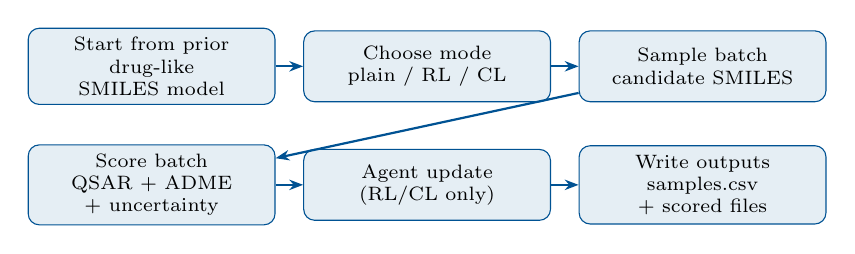
\begin{tikzpicture}[node distance=0.5cm and 0.35cm]
      \node[pstep] (r1) {Start from prior\\drug-like SMILES model};
      \node[pstep,right=of r1] (r2) {Choose mode\\plain / RL / CL};
      \node[pstep,right=of r2] (r3) {Sample batch\\candidate SMILES};
      \node[pstep,below=of r1] (r4) {Score batch\\QSAR + ADME + uncertainty};
      \node[pstep,right=of r4] (r5) {Agent update\\(RL/CL only)};
      \node[pstep,right=of r5] (r6) {Write outputs\\samples.csv + scored files};

      \draw[arrow] (r1)--(r2);
      \draw[arrow] (r2)--(r3);
      \draw[arrow] (r3)--(r4);
      \draw[arrow] (r4)--(r5);
      \draw[arrow] (r5)--(r6);
    \end{tikzpicture}
  \end{center}
\end{frame}

\begin{frame}{REINVENT4 modes and optimization details}
  \small
  \begin{tabularx}{\textwidth}{lX}
    \toprule
    \textbf{Mode} & \textbf{How optimization behaves} \\
    \midrule
    Plain & No policy update; broad exploration from prior distribution. \\
    RL & Iterative policy optimization from reward signal after scoring each batch. \\
    CL & Multi-stage objective: easier constraints first, stricter objectives later. \\
    Mol2Mol/LibINVENT/LinkINVENT & Family-specific generation constraints layered on top of training mode. \\
    \bottomrule
  \end{tabularx}

  \vspace{4pt}
  \begin{alertblock}{Why curriculum learning was used}
    It improves stability and validity while pushing toward higher-quality,
    multi-objective molecules under realistic constraints.
  \end{alertblock}
\end{frame}

\begin{frame}{REINVENT4 project execution and outputs}
  \begin{columns}[T]
    \column{0.50\textwidth}
      \begin{block}{What was run}
        \begin{itemize}
          \item Multiple generation families and modes
          \item Automated score pass after each sampling output
          \item Unified downstream gate ranking across all runs
        \end{itemize}
      \end{block}
    \column{0.48\textwidth}
      \begin{block}{Where outputs are saved}
        Raw samples:\\
        {\scriptsize\texttt{reinvent\_integration/results/<family\_mode>/samples.csv}}\\
        Scored results:\\
        {\scriptsize\texttt{outputs/generated/<family>/<mode>/}}
      \end{block}
  \end{columns}
\end{frame}

\begin{frame}{Generation activity scope in this project (not just 3 modes)}
  \small
  \begin{block}{Model families orchestrated in campaigns}
    reinvent, reinvent\_pubchem, pepinvent, mol2mol\_similarity,
    mol2mol\_high\_similarity, mol2mol\_medium\_similarity,
    mol2mol\_scaffold, mol2mol\_scaffold\_generic, mol2mol\_mmp,
    libinvent, libinvent\_transformer\_pubchem, linkinvent,
    linkinvent\_transformer\_pubchem, and the nitro\_bioisostere\_campaign.
  \end{block}

  \begin{exampleblock}{Operational implication}
    Each family was executed across plain/RL/CL flows with post-scoring, so
    the generation program is a \textbf{matrix of campaigns}, not a single run.
    Current generation coverage is fully populated across the targeted branches.
  \end{exampleblock}
\end{frame}

\begin{frame}{Generation campaign matrix: families \(\times\) optimization modes}
  \small
  \begin{tabularx}{\textwidth}{lccc}
    \toprule
    \textbf{Family group} & \textbf{Plain} & \textbf{RL} & \textbf{CL} \\
    \midrule
    REINVENT / REINVENT\_PubChem & \checkmark & \checkmark & \checkmark \\
    PepINVENT & \checkmark & \checkmark & \checkmark \\
    Mol2Mol (sim/high/medium/scaffold/scaffold\_generic/mmp) & \checkmark & \checkmark & \checkmark \\
    LibINVENT (+ transformer prior) & \checkmark & \checkmark & \checkmark \\
    LinkINVENT (+ transformer prior) & \checkmark & \checkmark & \checkmark \\
    Nitro bioisostere campaign & \checkmark & \checkmark & \checkmark \\
    \bottomrule
  \end{tabularx}

  \vspace{3pt}
  \begin{block}{Why this matrix matters}
    It separates exploration (plain), exploitation (RL), and robust staged optimization (CL),
    while covering multiple molecular design tasks (de novo, analoging, linking, decorating).
  \end{block}
\end{frame}

\begin{frame}{REINVENT / REINVENT\_PubChem (\checkmark \checkmark \checkmark)}
  \small
  \begin{columns}[T]
    \column{0.52\textwidth}
      \begin{block}{What this family contributes}
        \begin{itemize}
          \item Core de novo generation backbone
          \item REINVENT\_PubChem adds broader prior chemistry exposure
          \item Strong for novelty-first exploration
        \end{itemize}
      \end{block}
      \begin{block}{Modes in this project}
        \textbf{Plain}: baseline de novo sampling\\
        \textbf{RL}: reward-guided potency/ADME optimization\\
        \textbf{CL}: staged objective tightening for stable convergence
      \end{block}
    \column{0.46\textwidth}
      \begin{block}{Concrete run artifacts}
        Config examples:\\
        {\scriptsize\texttt{sample\_reinvent\_plain.toml}}\\
        {\scriptsize\texttt{rl\_reinvent.toml}} / {\scriptsize\texttt{cl\_reinvent.toml}}\\
        {\scriptsize\texttt{sample\_reinvent\_rl.toml}} / {\scriptsize\texttt{sample\_reinvent\_cl.toml}}\\[2pt]
        Raw outputs:\\
        {\scriptsize\texttt{reinvent\_integration/results/reinvent\_<mode>/samples.csv}}\\
        Scored outputs:\\
        {\scriptsize\texttt{outputs/generated/reinvent/<mode>/}}
      \end{block}
  \end{columns}
\end{frame}

\begin{frame}{PepINVENT (\checkmark \checkmark \checkmark)}
  \small
  \begin{columns}[T]
    \column{0.52\textwidth}
      \begin{block}{What this family contributes}
        \begin{itemize}
          \item Peptide-like sequence/structure generation focus
          \item Complements small-molecule-focused families
          \item Adds modality diversity to candidate pool
        \end{itemize}
      \end{block}
      \begin{block}{Modes in this project}
        \textbf{Plain}: broad peptide-like proposal space\\
        \textbf{RL}: prioritize higher reward peptide candidates\\
        \textbf{CL}: staged constraints to improve quality stability
      \end{block}
    \column{0.46\textwidth}
      \begin{block}{Concrete run artifacts}
        Config examples:\\
        {\scriptsize\texttt{sample\_pepinvent\_plain.toml}}\\
        {\scriptsize\texttt{rl\_pepinvent.toml}} / {\scriptsize\texttt{cl\_pepinvent.toml}}\\
        {\scriptsize\texttt{sample\_pepinvent\_rl.toml}} / {\scriptsize\texttt{sample\_pepinvent\_cl.toml}}\\[2pt]
        Raw outputs:\\
        {\scriptsize\texttt{reinvent\_integration/results/pepinvent\_<mode>/samples.csv}}\\
        Scored outputs:\\
        {\scriptsize\texttt{outputs/generated/pepinvent/<mode>/}}
      \end{block}
  \end{columns}
\end{frame}

\begin{frame}{Mol2Mol (sim/high/medium/scaffold/mmp) (\checkmark \checkmark \checkmark)}
  \small
  \begin{columns}[T]
    \column{0.54\textwidth}
      \begin{block}{What this family contributes}
        \begin{itemize}
          \item Controlled analog generation around references
          \item Multiple transformation regimes: similarity, scaffold, MMP
          \item Balances novelty with medicinal chemistry continuity
        \end{itemize}
      \end{block}
      \begin{block}{Modes in this project}
        \textbf{Plain}: analog exploration without policy updates\\
        \textbf{RL}: optimize transformations toward reward\\
        \textbf{CL}: staged analog objective tightening per regime
      \end{block}
    \column{0.44\textwidth}
      \begin{block}{Concrete run artifacts}
        Examples:\\
        {\scriptsize\texttt{sample\_mol2mol\_similarity\_plain.toml}}\\
        {\scriptsize\texttt{rl\_mol2mol\_high\_similarity.toml}}\\
        {\scriptsize\texttt{cl\_mol2mol\_scaffold.toml}}\\[2pt]
        Raw outputs:\\
        {\scriptsize\texttt{reinvent\_integration/results/mol2mol\_<variant>\_<mode>/samples.csv}}\\
        Scored outputs:\\
        {\scriptsize\texttt{outputs/generated/mol2mol/<variant>/<mode>/}}
      \end{block}
  \end{columns}
\end{frame}

\begin{frame}{LibINVENT (+ transformer prior) (\checkmark \checkmark \checkmark)}
  \small
  \begin{columns}[T]
    \column{0.52\textwidth}
      \begin{block}{What this family contributes}
        \begin{itemize}
          \item Scaffold decoration/library-style expansion
          \item Useful for R-group exploration at fixed cores
          \item Transformer prior variant broadens syntactic diversity
        \end{itemize}
      \end{block}
      \begin{block}{Modes in this project}
        \textbf{Plain}: enumerate baseline decoration ideas\\
        \textbf{RL}: improve decoration reward profile\\
        \textbf{CL}: staged decoration quality constraints
      \end{block}
    \column{0.46\textwidth}
      \begin{block}{Concrete run artifacts}
        Config examples:\\
        {\scriptsize\texttt{sample\_libinvent\_plain.toml}}\\
        {\scriptsize\texttt{rl\_libinvent.toml}} / {\scriptsize\texttt{cl\_libinvent.toml}}\\
        {\scriptsize\texttt{sample\_libinvent\_transformer\_pubchem\_cl.toml}}\\[2pt]
        Raw outputs:\\
        {\scriptsize\texttt{reinvent\_integration/results/libinvent\_<mode>/samples.csv}}\\
        {\scriptsize\texttt{reinvent\_integration/results/libinvent\_transformer\_pubchem\_<mode>/samples.csv}}
      \end{block}
  \end{columns}
\end{frame}

\begin{frame}{LinkINVENT (+ transformer prior) (\checkmark \checkmark \checkmark)}
  \small
  \begin{columns}[T]
    \column{0.52\textwidth}
      \begin{block}{What this family contributes}
        \begin{itemize}
          \item Linker design between anchors/fragments
          \item Critical for fragment-joining and geometry-aware assembly
          \item Transformer prior variant increases linker novelty breadth
        \end{itemize}
      \end{block}
      \begin{block}{Modes in this project}
        \textbf{Plain}: linker idea exploration\\
        \textbf{RL}: optimize linker candidates by reward\\
        \textbf{CL}: staged linker constraint tightening
      \end{block}
    \column{0.46\textwidth}
      \begin{block}{Concrete run artifacts}
        Config examples:\\
        {\scriptsize\texttt{sample\_linkinvent\_plain.toml}}\\
        {\scriptsize\texttt{rl\_linkinvent.toml}} / {\scriptsize\texttt{cl\_linkinvent.toml}}\\
        {\scriptsize\texttt{sample\_linkinvent\_transformer\_pubchem\_cl.toml}}\\[2pt]
        Raw outputs:\\
        {\scriptsize\texttt{reinvent\_integration/results/linkinvent\_<mode>/samples.csv}}\\
        {\scriptsize\texttt{reinvent\_integration/results/linkinvent\_transformer\_pubchem\_<mode>/samples.csv}}
      \end{block}
  \end{columns}
\end{frame}

\begin{frame}{Generation execution lifecycle (per family)}
  \begin{center}
    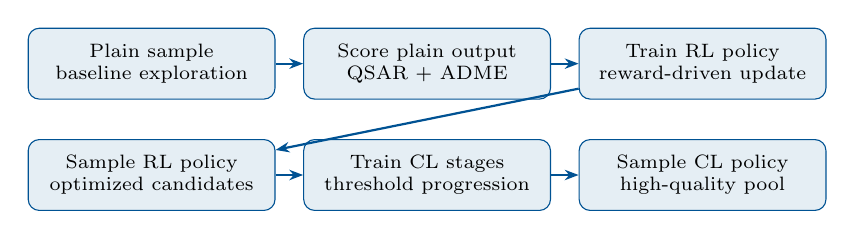
\begin{tikzpicture}[node distance=0.5cm and 0.35cm]
      \node[pstep] (e1) {Plain sample\\baseline exploration};
      \node[pstep,right=of e1] (e2) {Score plain output\\QSAR + ADME};
      \node[pstep,right=of e2] (e3) {Train RL policy\\reward-driven update};
      \node[pstep,below=of e1] (e4) {Sample RL policy\\optimized candidates};
      \node[pstep,right=of e4] (e5) {Train CL stages\\threshold progression};
      \node[pstep,right=of e5] (e6) {Sample CL policy\\high-quality pool};
      \draw[arrow] (e1)--(e2);
      \draw[arrow] (e2)--(e3);
      \draw[arrow] (e3)--(e4);
      \draw[arrow] (e4)--(e5);
      \draw[arrow] (e5)--(e6);
    \end{tikzpicture}
  \end{center}
\end{frame}

\begin{frame}{How run orchestration is implemented}
  \small
  \begin{block}{Controller scripts}
    \texttt{reinvent\_integration/run\_all\_generation.py}\\
    \texttt{reinvent\_integration/run\_all\_generation\_fast.py}\\
    \texttt{reinvent\_integration/run\_all\_generation\_strict.py}\\
    \texttt{reinvent\_integration/run\_nitro\_bioisostere\_campaign.py}
  \end{block}

  \begin{block}{Automated per-family sequence}
    For each family: plain sample \(\rightarrow\) score,
    RL train \(\rightarrow\) RL sample \(\rightarrow\) score,
    CL train \(\rightarrow\) CL sample \(\rightarrow\) score,
    then merge into hybrid stage-gate pipeline.
  \end{block}
\end{frame}

\begin{frame}{Diverse generation activities: family-specific intent}
  \small
  \begin{columns}[T]
    \column{0.48\textwidth}
      \begin{block}{Exploration and analoging}
        \begin{itemize}
          \item REINVENT / REINVENT\_PubChem: broad de novo novelty
          \item Mol2Mol similarity/high/medium: controllable analog search
          \item Mol2Mol scaffold/scaffold\_generic: scaffold-preserving design
          \item Mol2Mol MMP: matched-pair style transformations
        \end{itemize}
      \end{block}
    \column{0.48\textwidth}
      \begin{block}{Assembly and decoration tasks}
        \begin{itemize}
          \item PepINVENT: peptide-like sequence/structure design
          \item LinkINVENT: linker optimization between anchors
          \item LibINVENT: scaffold decoration libraries
          \item Transformer-PubChem variants: broader prior transfer
        \end{itemize}
      \end{block}
  \end{columns}
\end{frame}

\begin{frame}{Optimization depth: what RL and CL improve over plain}
  \small
  \begin{tabularx}{\textwidth}{lX}
    \toprule
    \textbf{Aspect} & \textbf{Practical behavior in pipeline} \\
    \midrule
    Potency targeting & RL/CL shift sampled distribution toward higher QSAR-ranked molecules. \\
    ADME alignment & Objective shaping increases fraction within preferred ADME windows. \\
    Feasibility control & CL staging reduces abrupt jumps that produce unstable candidates. \\
    Gate readiness & RL/CL outputs generally show better downstream Gate 1 shortlist quality. \\
    \bottomrule
  \end{tabularx}
\end{frame}

\begin{frame}{Generation run variants: default, fast, strict, campaign-specific}
  \small
  \begin{columns}[T]
    \column{0.48\textwidth}
      \begin{block}{Default/full campaign}
        Broad model matrix, full scoring stack,
        standard gate thresholds for ranked export.
      \end{block}
      \begin{block}{Fast variant}
        Reduced runtime profile for rapid iteration and sanity checks.
      \end{block}
    \column{0.48\textwidth}
      \begin{block}{Strict variant}
        Tighter constraints / stricter progression,
        useful for high-confidence candidate narrowing.
      \end{block}
      \begin{block}{Nitro bioisostere campaign}
        Focused chemistry campaign with dedicated configs and logs.
      \end{block}
  \end{columns}
\end{frame}

\begin{frame}{Generation logs: what information is captured}
  \small
  \begin{block}{Log locations and examples}
    \texttt{reinvent\_integration/logs/run\_all\_generation.log}\\
    \texttt{reinvent\_integration/logs/run\_all\_generation\_fast.log}\\
    \texttt{reinvent\_integration/logs/run\_all\_generation\_strict.log}\\
    Family logs: \texttt{<family>\_<mode>\_<train/sample>\_*.log}
  \end{block}

  \begin{block}{Operational signals extracted}
    \begin{itemize}
      \item step completion/failure status for each run
      \item training progress and sampling completion
      \item mode-specific checkpoints and campaign diagnostics
    \end{itemize}
  \end{block}
\end{frame}

\begin{frame}{Generation output hierarchy and handoff to scoring}
  \small
  \begin{columns}[T]
    \column{0.49\textwidth}
      \begin{block}{Raw generation outputs}
        \texttt{reinvent\_integration/results/<family>\_<mode>/samples.csv}\\
        plus campaign-level artifacts/checkpoints in results tree.
      \end{block}
    \column{0.49\textwidth}
      \begin{block}{Scored generation outputs}
        \texttt{outputs/generated/<family>/<mode>/}\\
        standardized scored files used by Gate 1 input pooling.
      \end{block}
  \end{columns}

  \vspace{3pt}
  \begin{exampleblock}{End-to-end linkage}
    Generation activity \(\rightarrow\) scoring normalization \(\rightarrow\)
    Gate 1 ranking \(\rightarrow\) scientist review and wet-lab planning.
  \end{exampleblock}
\end{frame}

\begin{frame}{REINVENT4 generation families: what each generates}
  \small
  \begin{tabularx}{\textwidth}{lX}
    \toprule
    \textbf{Family} & \textbf{Generation behavior and practical use} \\
    \midrule
    REINVENT (de novo) & Generates full molecules from learned prior; best for broad exploration. \\
    Mol2Mol & Starts from reference scaffold/seed and proposes close-but-improved analogs. \\
    LinkINVENT & Generates linkers to connect fragments while preserving anchor context. \\
    LibINVENT & Enumerates decoration vectors around a scaffold under reaction-like constraints. \\
    Transformer-PubChem variants & Broader pretraining bias for novelty and chemical grammar robustness. \\
    \bottomrule
  \end{tabularx}

  \vspace{4pt}
  \begin{exampleblock}{Project strategy}
    Use multiple families in parallel: broad exploration (de novo) + local optimization
    (scaffold/fragment-driven families), then merge all outputs into one scoring/gating path.
  \end{exampleblock}
\end{frame}

\begin{frame}{Plain generation details (exploration mode)}
  \begin{columns}[T]
    \column{0.50\textwidth}
      \begin{block}{What happens in plain mode}
        \begin{itemize}
          \item Agent weights are fixed (no optimization loop)
          \item Batched sampling from prior policy
          \item Strongly useful for baseline diversity
          \item Fast throughput for first-pass idea space
        \end{itemize}
      \end{block}
    \column{0.48\textwidth}
      \begin{block}{How outputs are used}
        \begin{itemize}
          \item Post-scored by QSAR + ADME pipeline
          \item Feeds Gate 1 diversity-aware shortlist
          \item Acts as discovery baseline vs RL/CL gains
        \end{itemize}
      \end{block}
  \end{columns}
\end{frame}

\begin{frame}{Reinforcement learning generation: optimization loop}
  \small
  \begin{center}
    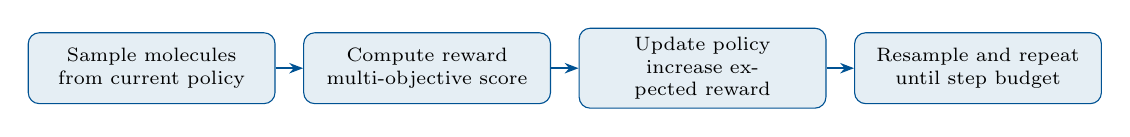
\begin{tikzpicture}[node distance=0.5cm and 0.35cm]
      \node[pstep] (rl1) {Sample molecules\\from current policy};
      \node[pstep,right=of rl1] (rl2) {Compute reward\\multi-objective score};
      \node[pstep,right=of rl2] (rl3) {Update policy\\increase expected reward};
      \node[pstep,right=of rl3] (rl4) {Resample and repeat\\until step budget};
      \draw[arrow] (rl1)--(rl2);
      \draw[arrow] (rl2)--(rl3);
      \draw[arrow] (rl3)--(rl4);
    \end{tikzpicture}
  \end{center}

  \vspace{3pt}
  \begin{block}{Optimization objective (conceptual)}
    \[
      J(\theta)=\mathbb{E}_{x\sim\pi_{\theta}}[R(x)]
      \quad \Rightarrow \quad
      \theta \leftarrow \theta + \eta\,\nabla_{\theta}J(\theta)
    \]
    Where \(R(x)\) combines potency, ADME, and feasibility/risk constraints.
  \end{block}
\end{frame}

\begin{frame}{Curriculum learning generation: staged optimization}
  \small
  \begin{columns}[T]
    \column{0.58\textwidth}
      \begin{block}{Why curriculum is stronger than single-stage RL}
        \begin{enumerate}
          \item Stage 1: satisfy validity/basic chemistry and minimal potency.
          \item Stage 2: tighten potency + key ADME windows.
          \item Stage 3: enforce full objective stack before final sampling.
        \end{enumerate}
        This reduces optimization collapse and improves final feasible hit-rate.
      \end{block}
    \column{0.40\textwidth}
      \begin{block}{Progression rule (conceptual)}
        Advance stage when:
        \[
        \bar{R}_{\text{window}} \ge \tau_s
        \]
        where \(\tau_s\) is stage threshold.
      \end{block}
  \end{columns}
\end{frame}

\begin{frame}{Reward construction used for REINVENT optimization}
  \small
  \begin{block}{Composite reward structure}
    \[
      R = w_p f_{\text{potency}} +
          w_s f_{\text{solubility}} +
          w_l f_{\log P} +
          w_m f_{\text{microsomal}} +
          w_h f_{t_{1/2}} -
          w_u f_{\text{uncertainty}} -
          w_t f_{\text{tox risk}}
    \]
    Positive terms drive efficacy/developability; penalty terms suppress unstable or risky candidates.
  \end{block}

  \begin{alertblock}{Important practical point}
    Generation optimization and gate triage are aligned but not identical:
    reward guides learning dynamics, gates enforce strict deployment filters.
  \end{alertblock}
\end{frame}

\begin{frame}{How to read REINVENT optimization quality in this project}
  \small
  \begin{columns}[T]
    \column{0.48\textwidth}
      \begin{block}{Healthy optimization signals}
        \begin{itemize}
          \item Mean score trend increases over steps
          \item Valid SMILES fraction stays high
          \item Diversity does not collapse too early
          \item Top candidates remain competitive in Gate 1 shortlist ranking
        \end{itemize}
      \end{block}
    \column{0.48\textwidth}
      \begin{block}{Warning patterns to monitor}
        \begin{itemize}
          \item Score spike with low diversity (mode collapse)
          \item Rising uncertainty in high-score molecules
          \item ADME out-of-window drift at later steps
          \item Weak Gate 1 shortlist enrichment ratio
        \end{itemize}
      \end{block}
  \end{columns}
\end{frame}

% ============================================================
\section{Gate 1 (Detailed)}
% ============================================================

\begin{frame}{Gate 1 flowchart: triage and diversity shortlist}
  \begin{center}
    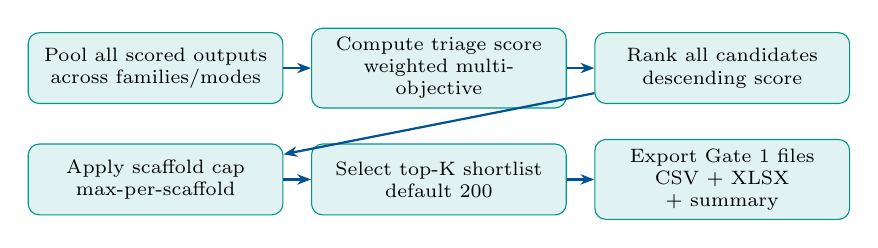
\begin{tikzpicture}[node distance=0.5cm and 0.35cm]
      \node[gatebox] (g1a) {Pool all scored outputs\\across families/modes};
      \node[gatebox,right=of g1a] (g1b) {Compute triage score\\weighted multi-objective};
      \node[gatebox,right=of g1b] (g1c) {Rank all candidates\\descending score};
      \node[gatebox,below=of g1a] (g1d) {Apply scaffold cap\\max-per-scaffold};
      \node[gatebox,right=of g1d] (g1e) {Select top-K shortlist\\default 200};
      \node[gatebox,right=of g1e] (g1f) {Export Gate 1 files\\CSV + XLSX + summary};

      \draw[arrow] (g1a)--(g1b);
      \draw[arrow] (g1b)--(g1c);
      \draw[arrow] (g1c)--(g1d);
      \draw[arrow] (g1d)--(g1e);
      \draw[arrow] (g1e)--(g1f);
    \end{tikzpicture}
  \end{center}
\end{frame}

\begin{frame}{Gate 1 details: scoring and output artifacts}
  \small
  \begin{block}{Triage equation}
    \[
    \text{triage}=0.35P+0.15S+0.15L+0.10M+0.10H+0.15T
    \]
    Potency is weighted highest; ADME balance and stability terms control quality.
  \end{block}

  \begin{block}{Gate 1 outputs}
    {\scriptsize\texttt{outputs/hybrid\_stage/gate1/gate1\_master\_ranked.csv}}\\
    {\scriptsize\texttt{outputs/hybrid\_stage/gate1/gate1\_shortlist.csv}}\\
    {\scriptsize\texttt{outputs/hybrid\_stage/gate1/gate1\_shortlist.xlsx}}\\
    {\scriptsize\texttt{outputs/hybrid\_stage/gate1/gate1\_summary.json}}
  \end{block}
\end{frame}

  \begin{frame}{Gate 1 shortlist: candidate pool composition (current)}
    \small
    \begin{columns}[T]
      \column{0.50\textwidth}
        \begin{block}{Source family breakdown (200 shortlisted)}
          \begin{tabularx}{\textwidth}{lr}
            \toprule
            \textbf{Family} & \textbf{Count} \\
            \midrule
            reinvent\_pubchem & 137 \\
            nitro\_bioisostere\_campaign & 53 \\
            reinvent & 9 \\
            linkinvent\_transformer\_pubchem & 1 \\
            \bottomrule
          \end{tabularx}
        \end{block}
      \column{0.48\textwidth}
        \begin{block}{Source mode breakdown}
          \begin{tabularx}{\textwidth}{lr}
            \toprule
            \textbf{Mode} & \textbf{Count} \\
            \midrule
            plain & 140 \\
            mol2mol\_similarity & 28 \\
            mol2mol\_scaffold\_generic & 22 \\
            curriculum\_learning & 6 \\
            mol2mol\_scaffold & 3 \\
            reinforcement\_learning & 1 \\
            \bottomrule
          \end{tabularx}
        \end{block}
    \end{columns}
    \vspace{3pt}
    \begin{exampleblock}{Observation}
      Plain-mode candidates dominate (70\%), with mol2mol analog variants
      contributing a significant diversity-preserving portion (26.5\%).
      Master ranked pool: \textbf{37,451} candidates from \textbf{14,287} unique scaffolds.
    \end{exampleblock}
  \end{frame}

% ============================================================
\section{Gate 2 / Gate 3 (Legacy, Inactive)}
% ============================================================

\begin{frame}{Gate 2 and Gate 3 status in current pipeline}
  \small
  \begin{alertblock}{Inactive stages}
    Gate 2 and Gate 3 are removed from the active implementation in
    \texttt{run\_hybrid\_stage\_gates.py}. Gate 1 is the only production stage.
  \end{alertblock}

  \begin{block}{How to interpret old references}
    \begin{itemize}
      \item Existing Gate 2/3 descriptions in legacy notes are historical context.
      \item Current ranked outputs are written only under \texttt{outputs/hybrid\_stage/gate1/}.
      \item Legacy folders remain for provenance in \texttt{outputs/hybrid\_stage/legacy/}.
    \end{itemize}
  \end{block}
\end{frame}

% ============================================================
\section{Why this project}
% ============================================================

\begin{frame}{Problem we are solving}
  \begin{block}{Goal}
    Start from many AI-generated molecules and end with a small, high-quality
    shortlist for laboratory testing.
  \end{block}

  \vspace{3pt}
  \begin{itemize}
    \item We do \textbf{not} have a reliable protein target structure for physics-heavy simulation.
    \item So we use a \textbf{target-free, data-driven pipeline}.
    \item We combine potency prediction, ADME quality, uncertainty, safety risk,
          and diversity before selecting final candidates.
  \end{itemize}

  \vspace{4pt}
  \begin{alertblock}{Business rationale}
    Reduce expensive false positives early, while keeping chemical diversity high.
  \end{alertblock}
\end{frame}

\begin{frame}{Core idea in one line}
  \begin{center}
    \Large
    Generate many molecules \(\rightarrow\) score quickly \(\rightarrow\)
    rank consistently \(\rightarrow\) prioritize for lab review
  \end{center}
\end{frame}

% ============================================================
\section{Key terms (plain language)}
% ============================================================

\begin{frame}{Key terms everyone should know}
  \begin{tabularx}{\textwidth}{lX}
    \toprule
    \textbf{Term} & \textbf{Simple meaning} \\
    \midrule
    SMILES & Text format for molecules (a way to write chemistry as strings). \\
    QSAR & Model that predicts activity/properties from structure. \\
    IC\(_{50}\) & Potency: lower value means stronger molecule. \\
    pIC\(_{50}\) & Log version of IC\(_{50}\): higher value means stronger molecule. \\
    ADME & Absorption, distribution, metabolism, excretion properties. \\
    Murcko scaffold & Core ring skeleton used to track diversity. \\
    Uncertainty & How much multiple good models disagree on prediction. \\
    \bottomrule
  \end{tabularx}
\end{frame}

\begin{frame}{Generation terms used in this project}
  \begin{tabularx}{\textwidth}{lX}
    \toprule
    \textbf{Term} & \textbf{Simple meaning} \\
    \midrule
    REINVENT (plain) & Generate molecules directly from pretrained chemistry language model. \\
    RL mode & Reinforcement learning: reward molecules with better predicted profile. \\
    CL mode & Curriculum learning: optimize in staged difficulty. \\
    Mol2Mol & Create analogs from seed molecules. \\
    LibINVENT & Decorate a scaffold with substituents. \\
    LinkINVENT & Connect fragments with designed linker. \\
    \bottomrule
  \end{tabularx}
\end{frame}

% ============================================================
\section{REINVENT 4 in this project}
% ============================================================

\begin{frame}{How REINVENT 4 generation modes work}
  \small
  \begin{tabularx}{\textwidth}{lX}
    \toprule
    \textbf{Mode} & \textbf{How it generates molecules} \\
    \midrule
    Plain (prior sampling) & Samples directly from pretrained chemical language model for broad exploration. \\
    RL (reinforcement learning) & Generates a batch, scores it, then updates the agent to prefer higher-scoring molecules. \\
    CL (curriculum learning) & Runs optimization in stages: easier objective first, then stricter objective later. \\
    Mol2Mol & Starts from known molecules and proposes close analogs. \\
    LibINVENT & Keeps a core scaffold and decorates attachment points with substituents. \\
    LinkINVENT & Connects two fragments with generated linkers. \\
    \bottomrule
  \end{tabularx}
\end{frame}

\begin{frame}{How curriculum learning optimization is done}
  \begin{columns}[T]
    \column{0.57\textwidth}
      \begin{block}{Optimization sequence}
        \begin{enumerate}
          \item Start from prior model (chemically valid baseline).
          \item Stage 1 objective: easier constraints (validity + broad quality).
          \item Stage 2 objective: stricter score (potency/ADME/uncertainty).
          \item At each step: sample \(\rightarrow\) score \(\rightarrow\) update agent.
          \item Stop at max steps or convergence, then sample final set.
        \end{enumerate}
      \end{block}
    \column{0.40\textwidth}
      \begin{block}{Why curriculum helps}
        \begin{itemize}
          \item More stable optimization
          \item Fewer invalid molecules
          \item Better quality-diversity tradeoff
          \item Less mode collapse
        \end{itemize}
      \end{block}
  \end{columns}
\end{frame}

\begin{frame}{How REINVENT 4 was used in this project}
  \small
  \begin{block}{What was done}
    Multiple generation families were run (including Mol2Mol, PepINVENT,
    LibINVENT, LinkINVENT and transformer variants) in one or more training
    modes (plain, RL, CL), then each sampled output was scored by the same
    QSAR + ADME + uncertainty pipeline.
  \end{block}

  \begin{columns}[T]
    \column{0.48\textwidth}
      \begin{block}{Execution flow}
        \begin{enumerate}
          \item Run REINVENT campaign config
          \item Write \texttt{samples.csv}
          \item Score via \texttt{score\_generated\_smiles\_adme.py}
          \item Save scored CSV/XLSX
        \end{enumerate}
      \end{block}
    \column{0.48\textwidth}
      \begin{block}{Where files are}
        \begin{itemize}
          \item Raw generations:\\
            \texttt{reinvent\_integration/results/}
          \item Scored outputs:\\
            \texttt{outputs/generated/<family>/<mode>/}
          \item Gate outputs:\\
            \texttt{outputs/hybrid\_stage/}
        \end{itemize}
      \end{block}
  \end{columns}
\end{frame}

\begin{frame}{REINVENT outputs that feed decision-making}
  \small
  \begin{block}{Per-run output}
    Each campaign produces generated SMILES plus scored tables containing
    potency, ADME, uncertainty, and source metadata.
  \end{block}

  \begin{block}{Cross-run integration}
    All scored runs are pooled and moved through:
    \begin{itemize}
      \item \textbf{Gate 1}: triage + scaffold-diverse top shortlist
      \item \textbf{Active stage}: Gate 1 only in the current workflow
      \item \textbf{Gate 2/3}: legacy reference only (inactive)
    \end{itemize}
  \end{block}

  \begin{exampleblock}{Final deliverable}
    A ranked candidate workbook with structures and rationale-ready fields,
    used by chemistry and biology teams for lab selection.
  \end{exampleblock}
\end{frame}

% ============================================================
\section{Process schema}
% ============================================================

\begin{frame}{End-to-end process schema}
  \begin{center}
    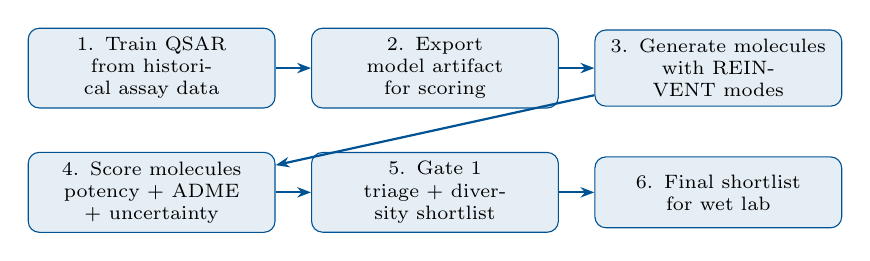
\begin{tikzpicture}[node distance=0.55cm and 0.45cm]
      \node[pstep] (s1) {1. Train QSAR\\from historical assay data};
      \node[pstep,right=of s1] (s2) {2. Export model artifact\\for scoring};
      \node[pstep,right=of s2] (s3) {3. Generate molecules\\with REINVENT modes};
      \node[pstep,below=of s1] (s4) {4. Score molecules\\potency + ADME + uncertainty};
      \node[pstep,right=of s4] (s5) {5. Gate 1\\triage + diversity shortlist};
      \node[pstep,right=of s5] (s8) {6. Final shortlist\\for wet lab};

      \draw[arrow] (s1)--(s2);
      \draw[arrow] (s2)--(s3);
      \draw[arrow] (s3)--(s4);
      \draw[arrow] (s4)--(s5);
      \draw[arrow] (s5)--(s8);
    \end{tikzpicture}
  \end{center}
\end{frame}

\begin{frame}{Active gate view (simple)}
  \begin{columns}[T]
    \column{0.60\textwidth}
      \begin{block}{Gate 1}
        \textbf{Fast triage}
        \begin{itemize}
          \item Potency + ADME
          \item Composite triage score
          \item Scaffold-diverse top 200
        \end{itemize}
      \end{block}
    \column{0.36\textwidth}
      \begin{alertblock}{Current status}
        Gate 2 and Gate 3 are retained only as historical references in older
        materials and are not active in the current production workflow.
      \end{alertblock}
  \end{columns}
\end{frame}

\begin{frame}{How scoring is carried out (step-by-step)}
  \small
  \begin{enumerate}
    \item \textbf{Validate SMILES} (remove invalid molecules).
    \item \textbf{Compute descriptors} from structure.
    \item \textbf{Predict potency} with best QSAR model.
    \item \textbf{Estimate uncertainty} from up to 5 positive-\(R^2\) models.
    \item \textbf{Add ADME / risk fields} (solubility, lipophilicity, clearance).
    \item \textbf{Apply gate logic} for ranking and filtering.
    \item \textbf{Export CSV + Excel} with structures for human review.
  \end{enumerate}

  \vspace{3pt}
  \begin{block}{Outcome}
    Every candidate has machine-scored evidence + a readable review format,
    so computational and chemistry teams can make the same decision from the
    same table.
  \end{block}
\end{frame}

% ============================================================
\section{How scoring is carried out (math)}
% ============================================================

\begin{frame}{Scoring mathematics: Gate 1 triage score}
  \small
  \begin{block}{Composite triage function}
  \[
  \text{triage} = 0.35\,P + 0.15\,S + 0.15\,L + 0.10\,M + 0.10\,H + 0.15\,T
  \]
  with\
  \(P\)=potency, \(S\)=solubility, \(L\)=cLogP window,
  \(M\)=microsomal clearance, \(H\)=hepatocyte clearance,
  \(T\)=half-life.
  \end{block}

  \begin{exampleblock}{Normalization}
  Higher-is-better:
  \[
  x_{norm}=\frac{x-x_{\min}}{x_{\max}-x_{\min}}
  \]
  Lower-is-better features are inverted after scaling.
  \end{exampleblock}
\end{frame}

\begin{frame}{Why these weights? (rationale)}
  \begin{itemize}
    \item \textbf{0.35 Potency}: strongest requirement; non-potent compounds are rarely useful.
    \item \textbf{0.30 Solubility + cLogP}: captures absorption/permeability balance.
    \item \textbf{0.20 Clearance terms}: avoids compounds that disappear too quickly in vivo.
    \item \textbf{0.15 Half-life}: rewards exposure duration without dominating the score.
  \end{itemize}

  \vspace{4pt}
  \begin{alertblock}{Important interpretation}
    This is a \textbf{triage utility score}, not a perfect biological truth.
    It is designed to rank candidates consistently for decision-making.
  \end{alertblock}
\end{frame}

\begin{frame}{How uncertainty is computed}
  \begin{block}{Model strategy}
    Keep the \textbf{best IC\(_{50}\)} model as primary prediction,
    then evaluate up to \textbf{five positive-\(R^2\)} models for the same molecule.
  \end{block}

  \begin{block}{Uncertainty proxy}
    Let predictions be \(\hat{y}_1,\hat{y}_2,\dots,\hat{y}_k\), \(k\leq 5\).
    \[
      \mu = \frac{1}{k}\sum_{i=1}^k \hat{y}_i,
      \quad
      \sigma = \sqrt{\frac{1}{k-1}\sum_{i=1}^k(\hat{y}_i-\mu)^2}
    \]
    Larger \(\sigma\) means lower confidence.
  \end{block}

  \begin{exampleblock}{Why it helps}
    Prevents over-prioritizing molecules that look strong in only one model.
  \end{exampleblock}
\end{frame}

\begin{frame}{Who carries out scoring? (roles in process)}
  \begin{tabularx}{\textwidth}{lX}
    \toprule
    \textbf{Role} & \textbf{What they do} \\
    \midrule
    REINVENT engine & Generates candidate SMILES across modes (plain/RL/CL). \\
    QSAR scoring script & Computes potency + ADME + uncertainty fields. \\
    Gate script & Applies triage math and diversity selection for Gate 1 shortlist generation. \\
    Medicinal chemist & Reviews computed outputs for structural quality and synthesis practicality. \\
    DMPK/safety scientist & Interprets computed tox/DDI/absorption risk outputs for go/no-go decisions. \\
    Project lead & Approves final shortlist for experiment. \\
    \bottomrule
  \end{tabularx}
\end{frame}

% ============================================================
\section{Repository map and outputs}
% ============================================================

\begin{frame}{Repository structure (current)}
  \begin{columns}[T]
    \column{0.50\textwidth}
      \begin{block}{Code folders}
        \begin{itemize}
          \item \texttt{qsar\_core/} core modules
          \item \texttt{reinvent\_integration/} generation + scoring + gates
          \item \texttt{scripts/} runnable scripts
          \item \texttt{config/} environment files
        \end{itemize}
      \end{block}
    \column{0.46\textwidth}
      \begin{block}{Data \& outputs}
        \begin{itemize}
          \item \texttt{data/raw/} input dataset
          \item \texttt{outputs/generated/} scored generations
          \item \texttt{outputs/hybrid\_stage/} gate outputs
          \item \texttt{docs/} plain-language documentation
        \end{itemize}
      \end{block}
  \end{columns}
\end{frame}

\begin{frame}{Main output files used in decisions}
  \small
  \begin{block}{1) Gate 1 shortlist (diversity + triage)}
    \texttt{outputs/hybrid\_stage/gate1/}\
    \texttt{gate1\_shortlist.xlsx}
  \end{block}

  \begin{block}{2) Gate 1 ranked table (full pool)}
    \texttt{outputs/hybrid\_stage/gate1/}\
    \texttt{gate1\_master\_ranked.csv}
  \end{block}

  \begin{block}{3) Legacy historical outputs (inactive stages)}
    \texttt{outputs/hybrid\_stage/legacy/}
  \end{block}
\end{frame}

% ============================================================
\section{Practical usage}
% ============================================================

\begin{frame}{How to run the pipeline (practical commands)}
  \begin{block}{From repository root}
    \begin{itemize}
      \item Export / refresh model artifact:\\
            {\scriptsize\texttt{python reinvent\_integration/export\_qsar\_model.py}}
      \item Run generation pipeline:\\
            {\scriptsize\texttt{python scripts/run\_pipeline.py}}
      \item Build stage-gated rankings:\\
            {\scriptsize\texttt{python reinvent\_integration/run\_hybrid\_stage\_gates.py}}
    \end{itemize}
  \end{block}

  \begin{exampleblock}{Preset options}
    {\scriptsize\texttt{python scripts/run\_pipeline.py --generation-preset fast|balanced|diverse}}
  \end{exampleblock}
\end{frame}

\begin{frame}{Decision logic summary}
  \begin{enumerate}
    \item Generate broad chemical space.
    \item Score with potency + ADME + uncertainty.
    \item Keep diversity while ranking quality.
    \item Remove uncertain / high-liability / hard-to-make molecules.
    \item Prioritize by Gate 1 triage score, diversity, and experiment value.
  \end{enumerate}

  \vspace{6pt}
  \begin{alertblock}{Why this works in no-target settings}
    It is fast, auditable, and aligned with real project decision gates,
    even when structure-based physics methods are unavailable.
  \end{alertblock}
\end{frame}

% ============================================================
\section{Excel field guide}
% ============================================================

\begin{frame}{How to read values in the Excel workbooks}
  \small
  \begin{columns}[T]
    \column{0.48\textwidth}
      \begin{block}{Binary / flag fields}
        \begin{itemize}
          \item \textbf{1} = passes / yes / valid / favorable
          \item \textbf{0} = fails / no / invalid / unfavorable
        \end{itemize}
        Active: \texttt{passes\_adme\_individual}, \texttt{passes\_adme\_ensemble},
        \texttt{passes\_optimal}, \texttt{passes\_metabolic\_stability}.\\
        Legacy (inactive): \texttt{passes\_gate2\_target\_free},
        \texttt{passes\_gate3\_translational}.
      \end{block}
      \begin{block}{Rank fields}
        \begin{itemize}
          \item Lower rank number = higher priority
          \item \texttt{rank} = Gate 1 order
          \item \texttt{gate2\_rank}, \texttt{gate3\_rank} = legacy inactive stages
        \end{itemize}
      \end{block}
    \column{0.48\textwidth}
      \begin{block}{Continuous score fields}
        \begin{itemize}
          \item Usually \textbf{higher = better} for composite scores
          \item Usually \textbf{lower = safer} for liabilities and uncertainty
          \item Always interpret with field meaning, not number alone
        \end{itemize}
      \end{block}
      \begin{exampleblock}{Key rule of thumb}
        \textbf{Higher potency score, higher confidence, higher absorption support}
        are good; \textbf{lower IC\(_{50}\), lower uncertainty, lower liability counts,
        lower toxicity/DDI risk} are good.
      \end{exampleblock}
  \end{columns}
\end{frame}

\begin{frame}{Gate 1 workbook fields: structure, potency, ADME, source}
  \scriptsize
  \begin{tabularx}{\textwidth}{lX}
    \toprule
    \textbf{Field} & \textbf{Meaning and value interpretation} \\
    \midrule
    \texttt{Structure} / \texttt{canonical\_smiles} & Molecule drawing / canonical text structure used for scoring and review. \\
    \texttt{SMILES\_state} & Validity flag; 1 means structurally accepted, 0 means invalid/problematic. \\
    \texttt{pred\_pIC50} & Predicted potency on log scale; higher means stronger predicted activity. \\
    \texttt{pred\_ic50\_uM} & Predicted potency in \(\mu\)M; lower means stronger predicted activity. \\
    \texttt{pred\_cLogP} & Predicted lipophilicity; mid-range is generally preferred over extreme low/high values. \\
    \texttt{pred\_logS\_ESOL} & Predicted solubility log scale; less negative / higher means more soluble. \\
    \texttt{pred\_MetStab\_Clearance\_Microsome\_AZ} & Microsomal clearance proxy; lower is generally better because slower clearance means better stability. \\
    \texttt{pred\_MetStab\_Clearance\_Hepatocyte\_AZ} & Hepatocyte clearance proxy; lower is generally better. \\
    \texttt{pred\_MetStab\_Half\_Life\_Obach} & Metabolic half-life proxy; higher means more stable / longer-lasting. \\
    \texttt{passes\_optimal}, \texttt{passes\_adme\_individual}, \texttt{passes\_adme\_ensemble} & Binary gate flags; 1 means the molecule is within the preferred rule window. \\
    \texttt{source\_family}, \texttt{source\_mode} & Which generator produced the compound and under which campaign mode. \\
    \bottomrule
  \end{tabularx}
\end{frame}

\begin{frame}{Gate 1 workbook fields: ranking and similarity}
  \scriptsize
  \begin{tabularx}{\textwidth}{lX}
    \toprule
    \textbf{Field} & \textbf{Meaning and value interpretation} \\
    \midrule
    \texttt{rank} & Gate 1 shortlist order; smaller rank means better overall triage priority. \\
    \texttt{triage\_score} & Main Gate 1 composite score; higher means better combined potency + ADME profile. \\
    \texttt{pred\_pIC50\_uncertainty} & Potency model disagreement; lower means higher confidence. \\
    \texttt{Input\_SMILES} & Original generator-provided structure string before normalization. \\
    \texttt{Tanimoto} & 2D structural similarity to the reference/seed context; higher means more similar, lower means more novel. \\
    \texttt{murcko\_scaffold} / \texttt{scaffold\_bucket} & Core chemotype grouping used to keep shortlist diversity. \\
    \texttt{adme\_ensemble\_score} & Ensemble ADME quality score combining solubility, lipophilicity, and metabolic stability; higher is better. \\
    \texttt{NLL} & Negative log-likelihood from generator; lower typically means the model finds the structure more probable. \\
    \bottomrule
  \end{tabularx}

  \vspace{2pt}
  \begin{exampleblock}{Observed Gate 1 behavior in current workbook}
    \texttt{triage\_score}: 0.77--0.92; \texttt{Tanimoto}: 0.28--0.86;
    \texttt{pred\_pIC50}: 4.94--6.11; \texttt{pred\_ic50\_uM}: 0.78--11.55\,\(\mu\)M.
  \end{exampleblock}
\end{frame}

\begin{frame}{Legacy Gate 2 workbook fields (inactive reference)}
  \scriptsize
  \begin{tabularx}{\textwidth}{lX}
    \toprule
    \textbf{Field} & \textbf{Meaning and value interpretation} \\
    \midrule
    \texttt{gate2\_target\_free\_score} & Gate 2 composite score; higher means stronger confidence + chemistry support. \\
    \texttt{passes\_gate2\_target\_free} & Binary Gate 2 pass flag; 1 means the molecule survives this refinement stage. \\
    \texttt{pred\_pIC50\_uncertainty} & Ensemble disagreement around potency; lower means more reliable prediction. \\
    \texttt{pred\_pIC50\_lower95} & Conservative lower confidence bound on potency; higher is better because even the lower bound remains active. \\
    \texttt{pred\_ic50\_uM\_upper95} & Conservative upper confidence bound in \(\mu\)M; lower is better. \\
    \texttt{uncertainty\_confidence\_score} & Confidence derived from uncertainty; higher means more trust in the potency estimate. \\
    \texttt{sa\_score} & Synthetic accessibility score; lower usually means easier to make. \\
    \texttt{sa\_accessibility} & Rescaled synthetic accessibility; higher means easier / more accessible synthesis. \\
    \texttt{liability\_alert\_count} & Count of chemistry alert motifs; lower is better. \\
    \texttt{liability\_free} & Binary alert-free flag; 1 means no detected alert motifs. \\
    \bottomrule
  \end{tabularx}
\end{frame}

\begin{frame}{Legacy Gate 2/3 workbook fields (inactive reference)}
  \scriptsize
  \begin{tabularx}{\textwidth}{lX}
    \toprule
    \textbf{Field} & \textbf{Meaning and value interpretation} \\
    \midrule
    \texttt{nearest\_active\_tanimoto}, \texttt{shape\_tanimoto\_max} & 2D/3D support from known actives; higher means stronger ligand-based support. \\
    \texttt{ligand\_support\_score} & Combined ligand evidence score; higher is better. \\
    \texttt{gate3\_translational\_score} / \texttt{experimental\_priority\_score} & Final experiment-priority scores; higher means better translational value. \\
    \texttt{tox\_safety\_score} & Combined toxicity safety summary; higher means safer overall profile. \\
    \texttt{ddi\_safety\_score} & Drug--drug interaction safety summary; higher means lower predicted DDI liability. \\
    \texttt{absorption\_score} & Combined absorption/permeability support; higher means better oral/transport potential. \\
    \texttt{hERG}, \texttt{DILI}, \texttt{ClinTox}, \texttt{AMES}, \texttt{Carcinogens\_Lagunin} & Risk probabilities/proxies; lower is safer because high values indicate more predicted toxicity concern. \\
    \texttt{max\_cyp\_inhibition} & Maximum CYP inhibition risk across enzymes; lower is safer for DDI liability. \\
    \texttt{HIA\_Hou}, \texttt{Bioavailability\_Ma}, \texttt{PAMPA\_NCATS} & Absorption-related probabilities/scores; higher is better. \\
    \texttt{Caco2\_Wang} & Cell permeability proxy; less negative / higher means better permeability. \\
    \bottomrule
  \end{tabularx}

  \vspace{2pt}
  \begin{alertblock}{Simple reading rule for the final workbook}
    Prefer molecules with \textbf{high} final priority / safety / absorption scores,
    but \textbf{low} uncertainty, alert count, toxicity risk, CYP inhibition risk,
    and predicted IC\(_{50}\).
  \end{alertblock}
\end{frame}

% ============================================================
\section{Tools used in this repository}
% ============================================================

\begin{frame}{Tools used in this repository: core modeling and generation}
  \scriptsize
  \begin{tabularx}{\textwidth}{lX}
    \toprule
    \textbf{Tool} & \textbf{Used for in this repo} \\
    \midrule
    \href{https://www.python.org/}{Python} & Main language for the full pipeline, orchestration scripts, QSAR training, scoring, and reporting. \\
    \href{https://numpy.org/}{NumPy} & Numeric arrays, descriptor matrices, statistics, and score calculations. \\
    \href{https://pandas.pydata.org/}{Pandas} & Reading Excel/CSV inputs, manipulating scored tables, exporting candidate workbooks. \\
    \href{https://www.rdkit.org/}{RDKit} & SMILES parsing, canonicalization, descriptors, fingerprints, scaffolds, similarity, and structure rendering. \\
    \href{https://github.com/mordred-descriptor/mordred}{Mordred} & Additional molecular descriptor generation for QSAR feature sets. \\
    \href{https://scikit-learn.org/}{scikit-learn} & Core QSAR regression models, preprocessing, comparison, and evaluation. \\
    \href{https://xgboost.readthedocs.io/}{XGBoost} / \href{https://lightgbm.readthedocs.io/}{LightGBM} / \href{https://catboost.ai/}{CatBoost} & Gradient-boosting model families benchmarked as candidate QSAR predictors. \\
    \href{https://github.com/MolecularAI/REINVENT4}{REINVENT4} & Molecular generation engine for de novo, RL, CL, Mol2Mol, LibINVENT, LinkINVENT, and PepINVENT campaigns. \\
    \bottomrule
  \end{tabularx}
\end{frame}

\begin{frame}{Tools used in this repository: scoring, visualization, and outputs}
  \scriptsize
  \begin{tabularx}{\textwidth}{lX}
    \toprule
    \textbf{Tool} & \textbf{Used for in this repo} \\
    \midrule
    \href{https://github.com/swansonk14/admet_ai}{ADMET-AI} & Predicted ADME/toxicity endpoints used in post-generation enrichment and shortlist annotations. \\
    RDKit SA\_Score & Synthetic accessibility estimation available for chemistry assessment features. \\
    \href{https://matplotlib.org/}{Matplotlib} / \href{https://seaborn.pydata.org/}{Seaborn} & Plots for QSAR distributions, cluster views, and reporting visuals. \\
    \href{https://jupyter.org/}{Jupyter Notebooks} & Exploratory analysis, debugging, and reproducible workflow inspection notebooks in the repo. \\
    Excel / workbook export & Final ranked candidate review tables with structures for chemistry/biology decision-making. \\
    \href{https://ctan.org/pkg/beamer}{LaTeX Beamer} & This presentation deck and PDF reporting output. \\
    External chemistry resources (for example \texttt{external\_tools/SwissMADE}) & Supporting reference/tooling assets stored alongside the workflow. \\
    \bottomrule
  \end{tabularx}

  \vspace{2pt}
  \begin{exampleblock}{Simple summary}
    The repo combines \textbf{cheminformatics} (RDKit, Mordred),
    \textbf{machine learning} (scikit-learn, boosting models),
    \textbf{molecular generation} (REINVENT4), and
    \textbf{developability scoring} (ADMET-AI + Gate 1 logic) into one pipeline.
  \end{exampleblock}
\end{frame}

\begin{frame}{What tools are used in the active Gate 1 workflow?}
  \small
  \begin{block}{Gate 1 tools}
    \begin{itemize}
      \item \href{https://www.rdkit.org/}{RDKit}: molecule handling, descriptors, scaffold logic
      \item \href{https://github.com/swansonk14/admet_ai}{ADMET-AI}: ADME/tox annotations used by scoring outputs
      \item QSAR ensemble utilities: potency prediction and uncertainty columns
      \item Pandas/NumPy: triage scoring, ranking, and shortlist selection
      \item \texttt{run\_hybrid\_stage\_gates.py}: builds Gate 1 ranked outputs
    \end{itemize}
  \end{block}

  \vspace{4pt}
  \begin{exampleblock}{Implementation file}
    Gate 1 is implemented in \texttt{reinvent\_integration/run\_hybrid\_stage\_gates.py}.
  \end{exampleblock}

  \begin{alertblock}{Important notes}
    Gate 2 and Gate 3 are not active in the current pipeline; older references
    remain only for provenance. Simulation Plus, GastroPlus, and ADMET Predictor
    are \textbf{not used} in the codebase and appear only as comparison examples
    in documentation.
  \end{alertblock}
\end{frame}

\begin{frame}{Thank you}
  \begin{center}
    \Large Questions?
  \end{center}
\end{frame}

\end{document}
